
\section{Architectural design}

Many areas of our project required decisions and a rationale behind it. These decisions are sorted by area below and each decision is explained shortly. In retrospect some of these decisions were less than optimal while others turned out great and a description of how these influenced our project and what we learned will be given. The first section consists of a short overview of the system and a graphic representation. The second section talks about our database-access-layer. The third section talks about our web-framework. The fourth section is about a collection of tools for automatic code generation. The last section describes the scheduler algorithm.

\subsection{Overview}
Our system is best understood as a web-application providing the functionality to access the automatic solver and manipulate the data related to scheduling... 

\begin{figure}[H]
	\centering
		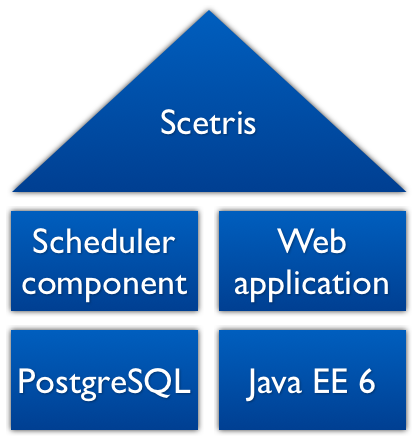
\includegraphics[width=0.5\textwidth]{images/scetris-house.png}
	\caption{\small An overview of the components}
	\label{fig:scetris-house}
\end{figure}

\subsection{Database access layer}

\emph{No existing solution but our own as we felt that existing solutions would take a similar amount of time to get used to and we would learn far more implementing the ORM ourselves. In regard to future work on the program, whether for maintenance or extension, it might prove beneficial to replace this solution with a more widely used tool, such as Hibernate. This would improve the process of understanding our software for people familiar with said tool. However we are satisfied with our own solution and we will stick with it, as it would be far too time-consuming to refactor this part of our project and we do not plan to work extensively with the software later on.}



\subsection{Web-framework}

\emph{Why we decided to use our own framework and how it is implemented. What the advantages are.}

We decided to implement our own web-framework as we wanted an easy integration of web-application and scheduling-algorithm. Thus a web-framework that uses the same language as our scheduling-algorithm was written to simplify the most common tasks. As well as getting a framework that fits our needs nicely, the benefit for us personally, which comes as knowledge was part of the reasoning against using an existing framework. We assume here that the knowledge of general principles is more beneficial to us than knowledge of tools.

\subsection{Tools for automatic code-generation}

\emph{Why a framework for common tasks has been created and how it affected our development process.}

As many tasks regarding the functionality of our web-interface require similar methods and should be implemented in a unified way to ease understanding, a framework for the most common tasks was written. It is called meta and is completely separated from the rest of our project, thus it can and will be used after we finished this project. So not only did it ease the development process for this project but also it will pay of even more in the long run.

\subsection{Scheduler Algorithm}
The problem of course scheduling is known to be NP-hard. The course scheduling problem can be approached by using search algorithms. As a matter of fact this works only for simple cases. Course scheduling, especially at universites and similiar big facilities, is faced with complex constraints. With the rise of input and more constraints finding an optimal solution cannot be computed in a sufficiently fast time. Based on several papers the approach of using a genetic algorithm is famous, seemed to be promising and was chosen therefore.

Genetic algorithm is a subset of metaheuristic optimization algorithm. Metaheuristics, being part of stochastic optimization, are algorithms using to some degree randomness in order to find optimal or as optimal as possible solutions to hard problems. Metaheuristics are applied when there is little to know about how the optimal solution looks like, there are to little heuristics to search on and brute-force is not questionable as the space of possible solution is to big. However when a candidate solution is given it can be scored in order to evaluate how good it is.

Typically a population of $\lambda$ number candidate solution is generated randomly, named \emph{setup}. The next step is an iteration containing the following process:

\begin{enumerate}
\item scoring the candidate solution by means of their \emph{fitness}

\item keeping only the $\mu$ best candidate solutions

\item generating new candidate solutions

	\begin{enumerate}
	\item selecting a candidate solution
	\item \emph{cross} it \emph{over} with another candidate solution
	\item \emph{mutate} the candidate solution
	\end{enumerate}
\end{enumerate}

To understand the the scheduler algorithm the genetic algorithm operations, \emph{setup}, \emph{fitness function}, \emph{crossover}, \emph{mutate} and \emph{selection} are best understood in means of core components of the scheduler algorithm. These operations are described below.

\begin{description}
\item[Setup] generates the initial population of candidate solutions in a random or semi-random way. A candidate solution is created when every course is allocated in a room at a given time. The \emph{setup} process is finished when $\lambda$ candidate solutions were created.

\item[Fitness function] evaluates the candidate solution by scoring it. The score is mapped to the number of constraints satisfied. The more constraints are satisfied the higher the candidate solution is scored. The score reaches from $0.0$ to $1.0$.

\item[Crossover] creates a new candidate solution by mixing and matching parts of two given candidate solution. How the mixing and matching is done relies on the representation of a candidate solution. As our representation is a mapping from courses to allocated room and time, these allocations are mixed and matched.

\item[Mutation] creates a new candidate solution by taking a given candidate solution and changing a specified amount of course allocations to new, randomly chosen, course allocations.

\item[Selection] iterates the given candidate solutions and keeps only the $\mu$ best solutions. The solutions are selected, according to the score given by the \emph{fitness function}, through dropping the rest of the candidate solutions.
\end{description}

The problem of course scheduling is defined by the given constraints which have to be satisfied. In order to meet the MyCourses specification requirements of high configurability we distinguish constraints by \emph{hard} and \emph{soft constraints}.

\begin{description}
\item[Hard constraints] are constraints which have to be satisfied. If these constraints are not satisfied the lecturing of courses is not possible. This includes the following constraints:

\begin{itemize}
\item not more than 1 course in the same room at the same time

\item the course lecturer has no other course at the same time

\item courses belonging to the same year do not overlap with each other in time in order to guarantee studiability

\item every constraint defined by the user with the priority of $100\%$, for instance preferred time, preferred room, etc.
\end{itemize}

\item[Soft constraints] are constraints which do not have to be ultimately satisfied. This includes only constraints defined by the user with a priority less than $100\%$.
\end{description}

An \emph{optimal solution} is a scheduling which asserts the satisfaction of all \emph{hard} and \emph{soft} constraints. Respectively the schedules score for \emph{hard} and \emph{soft fitness} is both $1.0$.

In the implementation phase it turned out using a \emph{setup} allocating the course completely random works for little input very well. With increased input, however, the results by  the classical \emph{setup} lead to quiet worse results. These results are supposed to be optimized by the phase of applying \emph{crossover} and \emph{mutate}. As a matter of fact this happens to a certain degree but starts to converging to a certain score.

Therefore an alternative \emph{setup} was implemented. \emph{Greedy setup} combines the approach of a genetic algorithm using metaheuristic with the Greedy algorithm being a subset of the combinatorial algorithm.

\begin{description}
\item[Greedy Setup] generates the initial population of candidate solutions by using a Greedy algorithm. Every course is allocated by placing it to the room which fits its constraints the best, for instance the requirement for a specified amount of seats. In order to avoid choosing rooms which exceed the required constraints every room is scored and sorted. In order to avoid overlapping in space and time the courses are place one after another in the timetable.
\end{description}

Figure \ref{fig:scheduler} illustrates the components interaction. At the start of each scheduling a initial population containing $\lambda$ possible schedule solutions is generated by \emph{Greedy Setup}. Randomly chosen courses are placed into the room which fits the course constraints the best. In this step the time slots are chosen at the earliest possible time slot and are distributed along all days at the week. If, however, there is a constraint for a preferred room or a preferred time slot entered by the user this spot is chosen directly.

\begin{figure}[H]
	\centering
		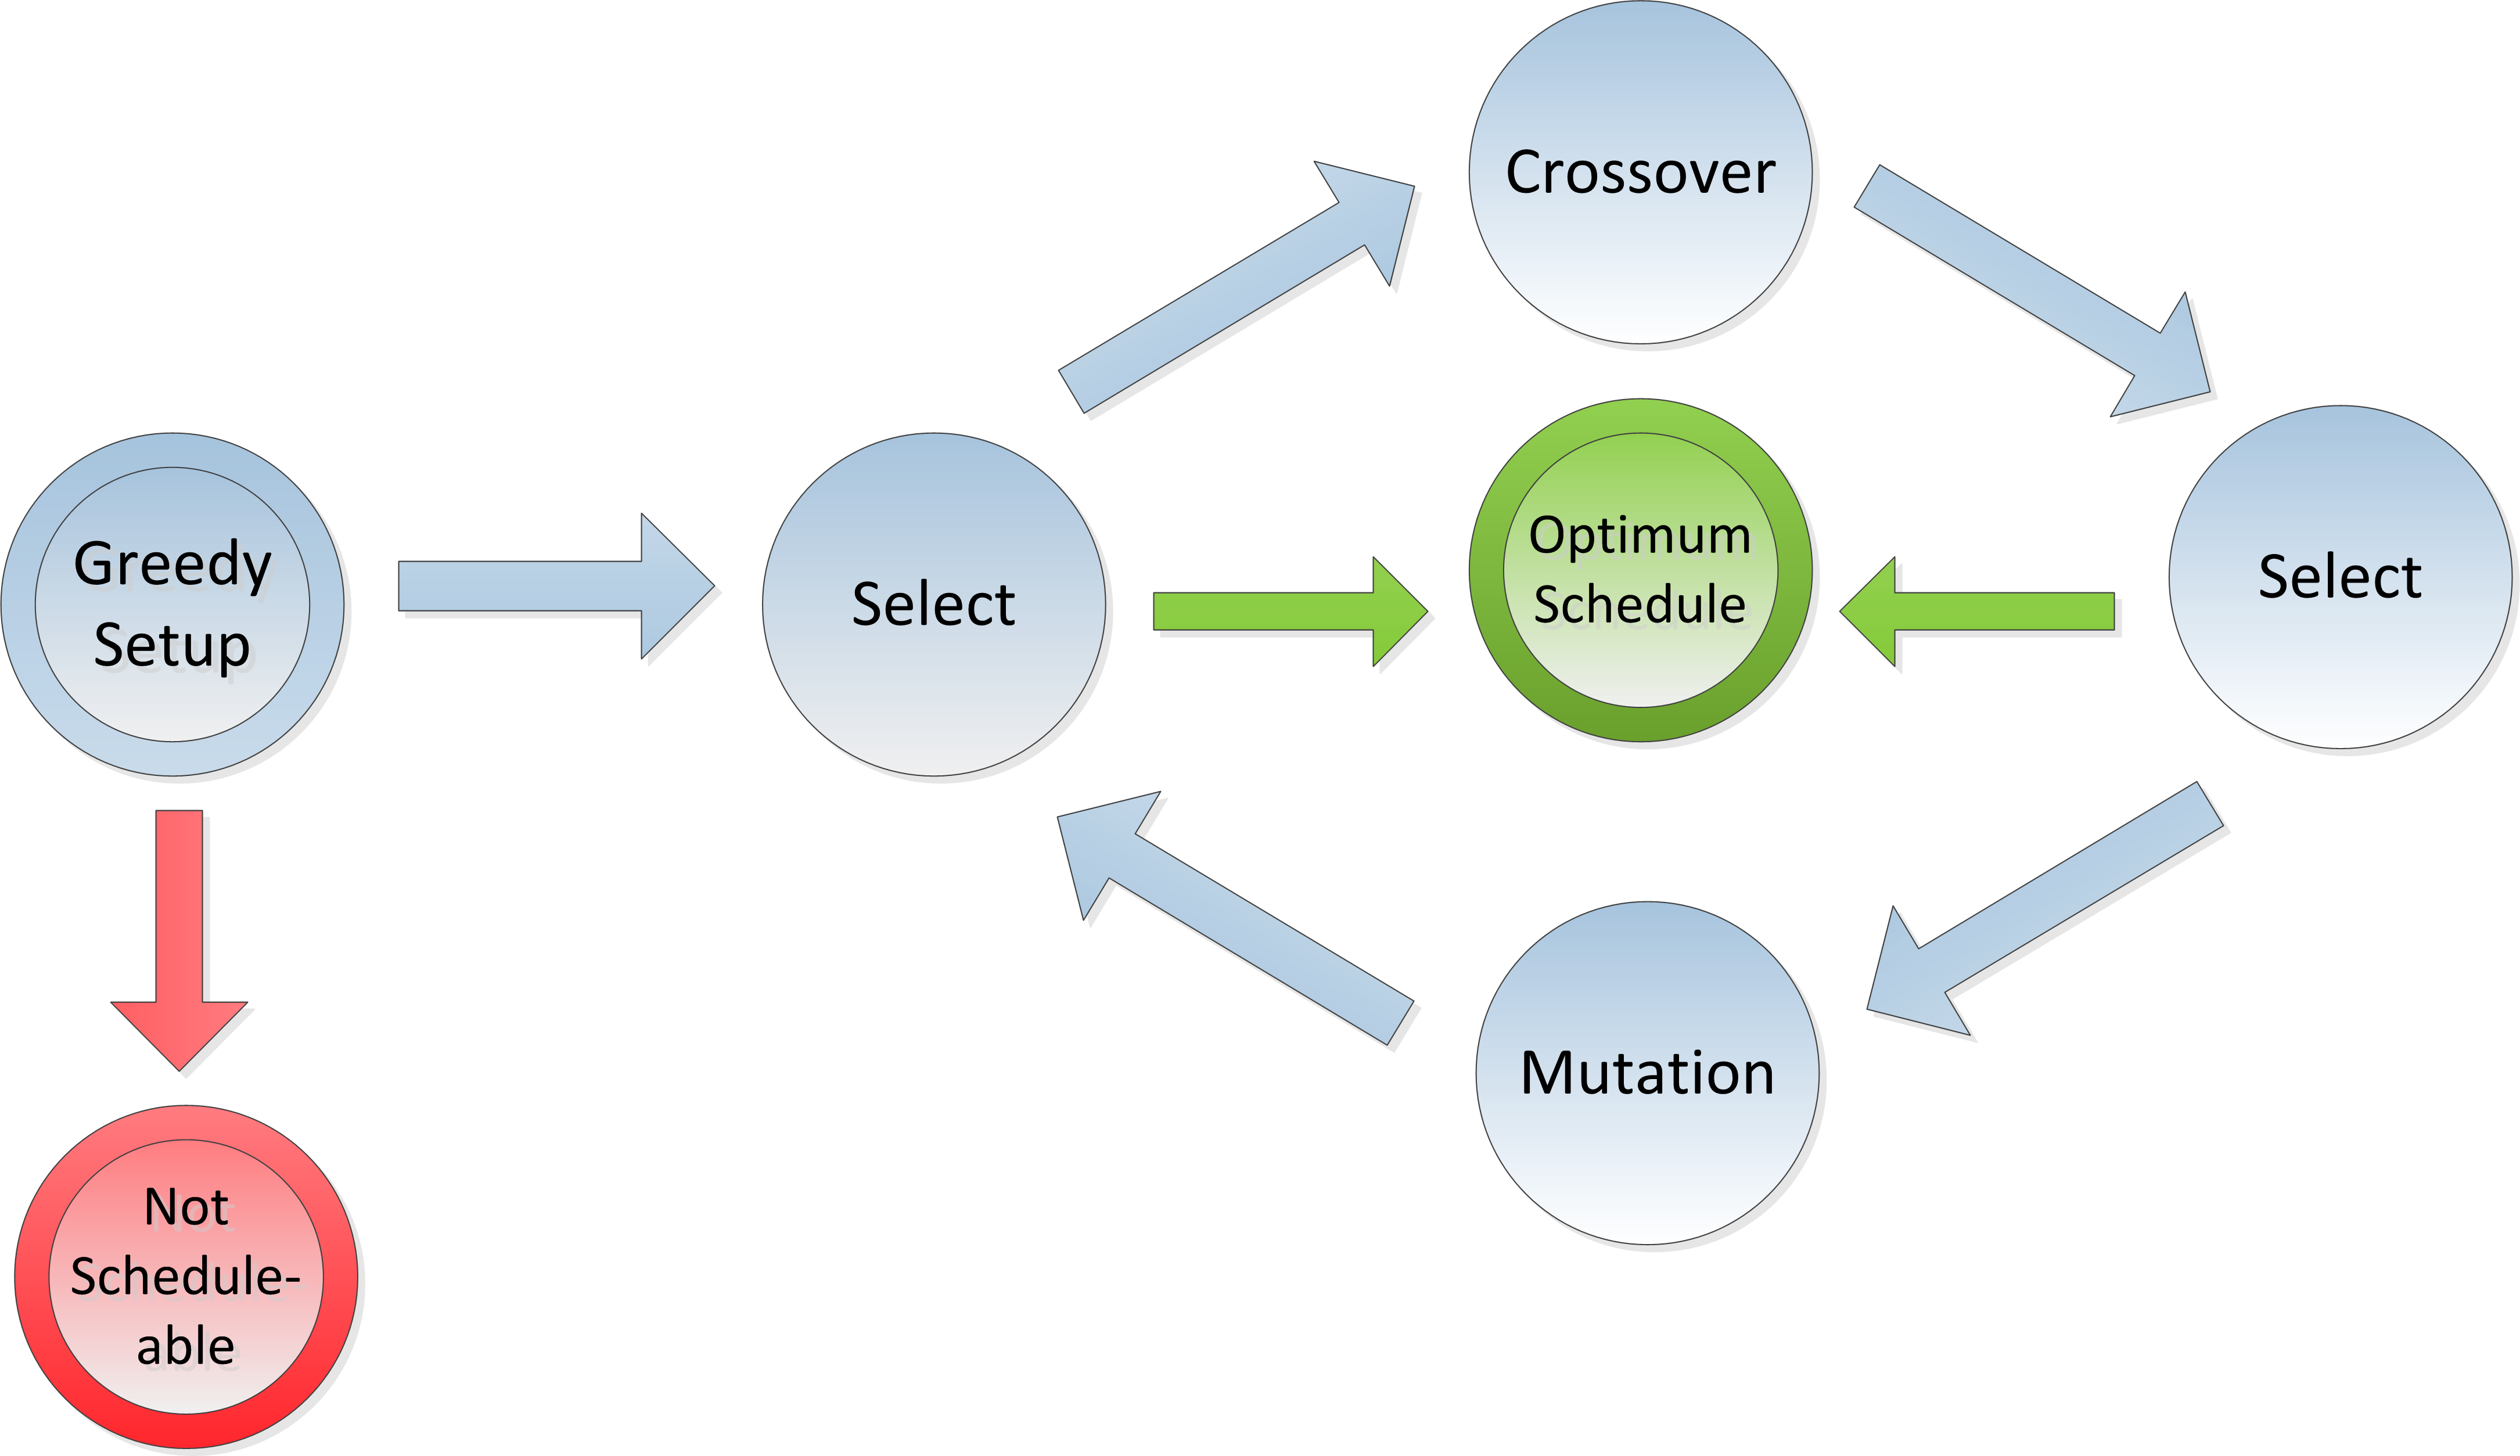
\includegraphics[width=\textwidth]{images/scheduler.png}
	\caption{Routine of the scheduler algorithm. Greedy Setup generates a initial population of candidate solutions. Every candidate solution is scored. If non-solvable conflicts appear the scheduling has to be terminated by means of not being scheduleable. Otherwise the Setup phase is followed by optimizing the candidate solutions by applying crossover and mutation operation until an optimum schedule is found.}
	\label{fig:scheduler}
\end{figure}

There is the possibility of finding an optimal solution in the phase of \emph{Greedy setup}. Therefore the \emph{fitness function} is applied on every generated candidate solution. If a optimal schedule was found the algorithm has terminated.


It is also possible the wished scheduling is not scheduleable at all. For instance when two course have the hard constraint to be placed at the same room with overlapping time. In this case the scheduling is stopped and the user has to resolve the constraint conflict by himself.

Otherwise the \emph{Greedy setup} will complete and the iteration of applying \emph{crossover}, \emph{mutation} and \emph{select} operation is started.  After each \emph{crossover} and \emph{mutation} only the best $\mu$ candidate solutions are kept and are tested for reaching the score $1.0$ which would lead to the algorithm termination.

